\documentclass[12pt]{article}\usepackage[]{graphicx}\usepackage[]{color}
%% maxwidth is the original width if it is less than linewidth
%% otherwise use linewidth (to make sure the graphics do not exceed the margin)
\makeatletter
\def\maxwidth{ %
  \ifdim\Gin@nat@width>\linewidth
    \linewidth
  \else
    \Gin@nat@width
  \fi
}
\makeatother

\definecolor{fgcolor}{rgb}{0.345, 0.345, 0.345}
\newcommand{\hlnum}[1]{\textcolor[rgb]{0.686,0.059,0.569}{#1}}%
\newcommand{\hlstr}[1]{\textcolor[rgb]{0.192,0.494,0.8}{#1}}%
\newcommand{\hlcom}[1]{\textcolor[rgb]{0.678,0.584,0.686}{\textit{#1}}}%
\newcommand{\hlopt}[1]{\textcolor[rgb]{0,0,0}{#1}}%
\newcommand{\hlstd}[1]{\textcolor[rgb]{0.345,0.345,0.345}{#1}}%
\newcommand{\hlkwa}[1]{\textcolor[rgb]{0.161,0.373,0.58}{\textbf{#1}}}%
\newcommand{\hlkwb}[1]{\textcolor[rgb]{0.69,0.353,0.396}{#1}}%
\newcommand{\hlkwc}[1]{\textcolor[rgb]{0.333,0.667,0.333}{#1}}%
\newcommand{\hlkwd}[1]{\textcolor[rgb]{0.737,0.353,0.396}{\textbf{#1}}}%

\usepackage{framed}
\makeatletter
\newenvironment{kframe}{%
 \def\at@end@of@kframe{}%
 \ifinner\ifhmode%
  \def\at@end@of@kframe{\end{minipage}}%
  \begin{minipage}{\columnwidth}%
 \fi\fi%
 \def\FrameCommand##1{\hskip\@totalleftmargin \hskip-\fboxsep
 \colorbox{shadecolor}{##1}\hskip-\fboxsep
     % There is no \\@totalrightmargin, so:
     \hskip-\linewidth \hskip-\@totalleftmargin \hskip\columnwidth}%
 \MakeFramed {\advance\hsize-\width
   \@totalleftmargin\z@ \linewidth\hsize
   \@setminipage}}%
 {\par\unskip\endMakeFramed%
 \at@end@of@kframe}
\makeatother

\definecolor{shadecolor}{rgb}{.97, .97, .97}
\definecolor{messagecolor}{rgb}{0, 0, 0}
\definecolor{warningcolor}{rgb}{1, 0, 1}
\definecolor{errorcolor}{rgb}{1, 0, 0}
\newenvironment{knitrout}{}{} % an empty environment to be redefined in TeX

\usepackage{alltt}

% packages
\usepackage{geometry}
\usepackage{amsmath}
\usepackage{amsfonts}
\usepackage{enumitem}
\usepackage{graphicx}
\usepackage{noweb}


\newcommand{\Q}[1]{\subsection*{Q.#1}}
\newenvironment{question}[1]
{\Q{#1}}{}


\newcommand{\union}[1]{\underset{#1}{\cup} }
\newcommand{\bigunion}[1]{\underset{#1}{\bigcup} \, }
\newcommand{\inter}[1]{\underset{#1}{\cap} }
\newcommand{\biginter}[1]{\underset{#1}{\bigcap} }
\newcommand{\minimize}[3]{\optimize{#1}{#2}{#3}{min}}
\newcommand{\maximize}[3]{\optimize{#1}{#2}{#3}{max}}
\newcommand{\esp}{{\mathbb E}}
\newcommand{\pr}{{\mathbb P}}
\newcommand{\norm}[1]{\Vert #1 \Vert}
\newcommand{\fnorm}[1]{\Vert #1 \Vert_F}
\newcommand{\nucnorm}[1]{\Vert #1 \Vert_*}
\newcommand{\opnorm}[1]{\Vert #1 \Vert_{op}}
\newcommand{\inner}[2]{\langle #1 \, , \, #2 \rangle}

\DeclareMathOperator{\cov}{cov}
\DeclareMathOperator{\var}{var}
\DeclareMathOperator{\err}{err}
\DeclareMathOperator{\tr}{tr}
\DeclareMathOperator{\rank}{Rank}
\DeclareMathOperator{\conv}{conv}


% parameters
\geometry{hmargin=1.5cm,vmargin=1.5cm}
\title{ORF525 - Problem Set 1}
\author{Bachir EL KHADIR }
\IfFileExists{upquote.sty}{\usepackage{upquote}}{}
\begin{document}
\maketitle

\begin{question}{1}

  \begin{enumerate}
  \item The conversion is necessary because otherwise we would have an unwanted order relation. For three similar houses A, B, C in zipcodes 98001, 98002, 98003, a linear model would be forced to affect a price for the house A that lies between the price for house A and C, which is a bug and not a future of the data itself.

\begin{knitrout}
\definecolor{shadecolor}{rgb}{0.969, 0.969, 0.969}\color{fgcolor}\begin{kframe}
\begin{alltt}
\hlstd{train.data} \hlkwb{<-} \hlkwd{read.csv}\hlstd{(}\hlstr{'data/train.data.csv'}\hlstd{)}
\hlstd{test.data} \hlkwb{<-} \hlkwd{read.csv}\hlstd{(}\hlstr{'data/test.data.csv'}\hlstd{)}
\hlstd{train.data}\hlopt{$}\hlstd{zipcode} \hlkwb{<-} \hlkwd{as.factor}\hlstd{(train.data}\hlopt{$}\hlstd{zipcode)}
\hlstd{test.data}\hlopt{$}\hlstd{zipcode} \hlkwb{<-} \hlkwd{as.factor}\hlstd{(test.data}\hlopt{$}\hlstd{zipcode)}
\end{alltt}
\end{kframe}
\end{knitrout}

\item
\begin{knitrout}
\definecolor{shadecolor}{rgb}{0.969, 0.969, 0.969}\color{fgcolor}\begin{kframe}
\begin{alltt}
\hlstd{linear.model} \hlkwb{<-} \hlkwd{lm}\hlstd{(price} \hlopt{~} \hlstd{bedrooms} \hlopt{+} \hlstd{bathrooms} \hlopt{+} \hlstd{sqft_living} \hlopt{+} \hlstd{sqft_lot,}
\hlkwc{data}\hlstd{=train}\hlopt{$}\hlstd{data)}
\end{alltt}


{\ttfamily\noindent\bfseries\color{errorcolor}{\#\# Error in is.data.frame(data): object 'train' not found}}\end{kframe}
\end{knitrout}

    \begin{enumerate}
    \item[a)]
      
      
    \item[b)]
    \end{enumerate}

  \end{enumerate}
\end{question}

\begin{question}{2}
  \begin{itemize}
  \item 
  $\Vert Y - \theta\Vert _2^2 + 4\tau^2 \Vert \theta\Vert _0 = \sum (y_i - \theta_i)^2 + 4\tau^2 1_{\theta_i \ne 0} = \sum_i f(\theta_i)$
  Where $f: \theta \rightarrow (y - \theta)^2 + 4\tau^2 1_{\theta \ne 0}$, eg
  \[
    f(\theta) = \left\{
      \begin{array}{cc}
        y^2 & \text{if } \theta = 0\\
        (y - \theta)^2 + 4 \tau^2& \text{if } \theta \ne 0\\
      \end{array}
    \right.
  \]
  The problem is linearly separable, we can minimize on each variable
  $\theta_i$ independetly:
  \begin{itemize}
  \item If $|y| > 2\tau$, then $y^2 \ge 4\tau^2$ and
    $(y - \theta)^2 + 4\tau^2 \ge 4\tau^2 = f(y)$.
  \item If $|y| \le 2\tau$, then
    $f(0) = y^2 \le 4\tau^2 \le y^2 + (y-\theta) = f(\theta) \forall
    \theta \ne 0$.
  \end{itemize}
  So
  $\arg\min \Vert Y - \theta\Vert _2^2 + 4\tau^2 = \hat
  \theta^{\text{hard}}$.
  
\item 
  $$ \Vert Y - \theta\Vert _2^2 + 4\tau \Vert \theta\Vert _1 = \sum
  (y_i - \theta_i)^2 + 4\tau |\theta_i| = \sum_i g(\theta_i)
  $$

  The problem is linearly separable, we can minimize on each variable
  $\theta_i$ independetly.
  $g: \theta \rightarrow (y - \theta)^2 + 4\tau |\theta|$, eg
  \[
    g(\theta) = \left\{
      \begin{array}{ccc}
        g_1(\theta) = (y - \theta)^2 + 4 \tau \theta&= (\theta - (-2\tau+y) )^2 + 2\tau(\tau+y) & \text{if } \theta \ge 0\\
        g_2(\theta) = (y - \theta)^2 - 4 \tau \theta&= (\theta - (2\tau+y) )^2 + 2\tau(\tau+y)  & \text{if } \theta \le 0\\
      \end{array}
    \right.
  \]



  \begin{itemize}
  \item
    \begin{itemize}
    \item If $|y| \le 2\tau$, then $g_1$ is increasing on  $[0, \infty)$, so it has a minimum at $0$, and the minimum is   $y^2 = g(0)$.
    \item   $g_2$ is decreasing on $(-\infty, 0]$ so it has a  minimum at 0.
    \item   c/c $\arg\min g$ in this case is 0.
    \end{itemize}

  \item
    \begin{itemize}
    \item If $y \ge 2\tau$ then $g_1$ has minimum at $y - 2\tau > 0$  and the minimum is $ y^2 - (2\tau-y)^2$.
    \item   $g_2$ is decreasing  and has a minimum at 0, $g_2(0) = y^2 \ge g(y-2\tau)$ with equality only if $y-2\tau = 0$
    \item c/c  $\arg\min g$ in this case is $y - 2\tau$.
    \end{itemize}

  \item if $y \le -2\tau$, by a similar argument, $\arg\min g$ in this
    case is $y - 2\tau$.
  \end{itemize}
  
  So
  $\arg\min \Vert Y - \theta\Vert _2^2 + 4\tau \theta = \hat
  \theta^{\text{hard}}$.
\end{itemize}
\end{question}
\begin{question}{3}
  \begin{enumerate}
  \item 

    \begin{figure}[ht]
      \centering
      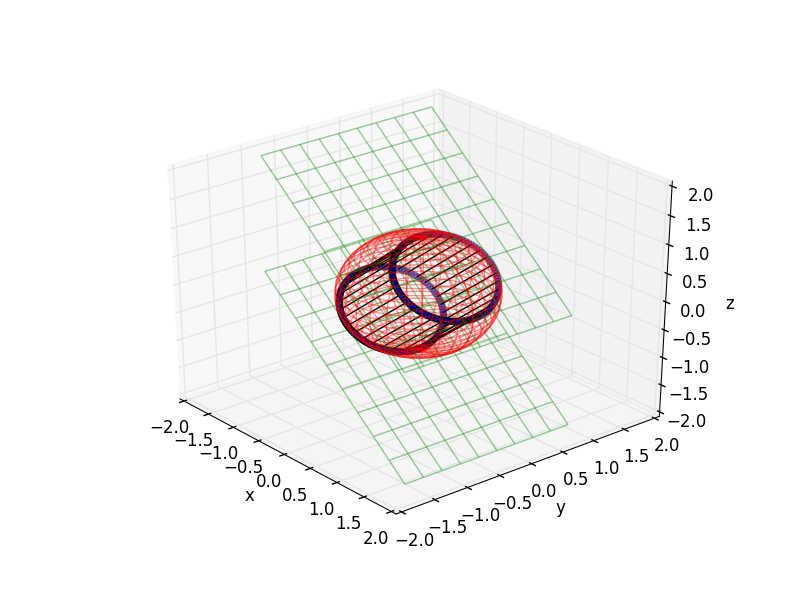
\includegraphics[scale=0.4]{nucnormset1.png}
      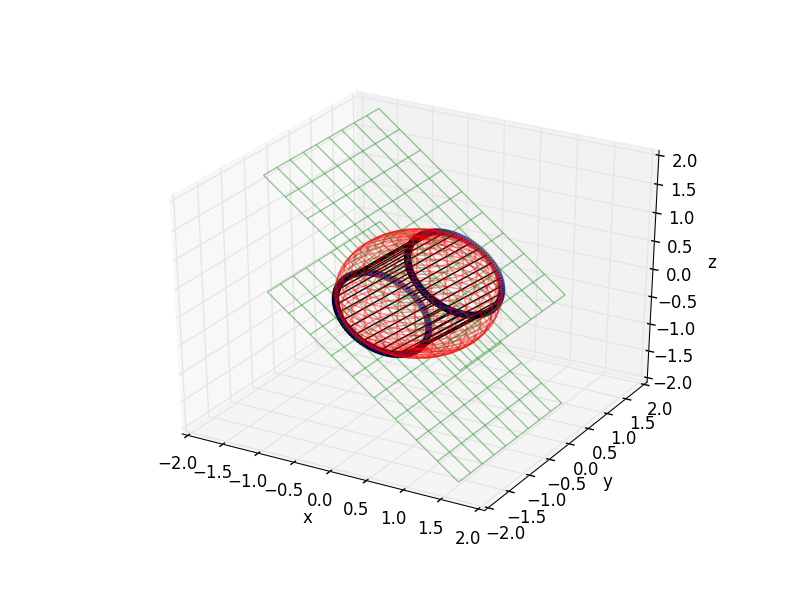
\includegraphics[scale=0.4]{nucnormset2.png}
      \caption{\label{fig:q3} Set}
    \end{figure}

    \begin{enumerate}
    \item
      $M(x,y,z)$ is of rank 1, so $(x y)$ and $(y z)$ are colinear, so  $ \exists \lambda  \in \mathbb{R} \; (x y) = \lambda (y z)  \text{ or } (y z) = \lambda (z y)$
      \begin{enumerate}
      \item Let's assume that $(x y) = \lambda (y z)$, and we can
        deduce the other case by symmetry.  In this case
        $x = \lambda^2 z, y = \lambda z$. Which means that $y^2 = \lambda^2z z = xz$.
      \item When $(y z) = \lambda (x y)$, by a similar argument, $y^2 = xz$
      \end{enumerate}
      The op norm is the biggest eigen value in absolute value, in this case since one of the
      eigen values is 0 (because the determinant is 0) the op norm is:
      $|tr(M(x, y, z))| = |x + z|$, this is equal to 1 only if $1 = |x+z|^2 = x^2 + z^2 + 2xz = x^2 + z^2 + 2y^2$
      Letting $t = \sqrt y$, we have that:
      $\{ (x, \sqrt2 y, z) | \rank(M) = 1, \Vert M\Vert _{op} = 1 \} \subseteq \{ (x, t, z): x^2 + t^2 + z^2 = 1, |x+z|=1  \} $


      
      For a matrix $M(x, y, z)$ such that $x^2 + z^2 + 2y^2 = 1$ and $|x+z|=1$, it is easy to see that:
      \begin{itemize}
      \item $\Vert M\Vert _{op} = |\tr(M)| = |x+z| = 1$
      \item $y^2 = \frac{1 - x^2 + z^2}2 = \frac{(x+z)^2 - x^2 - y^2}2 = xz$, so $\det(M) = 0$, therefore $M$ cannot have rank 2. It cannot have rank 0 either because $x^2 + 2y^2 + z^2 = 1 \implies$ one of the coefficient is not 0.
      \end{itemize}
      Therefore we have:
      $\{ (x, \sqrt2 y, z) | \rank(M) = 1, \Vert M\Vert _{op} = 1 \} = \{ (x, t, z): x^2 + t^2 + z^2 = 1, |x+z|=1  \} $
      
      $x^2 + t^2 + z^2$ describes the unit sphere, $|x+z| = 1$ describe the union of the two hyperplanes $x + z = \pm 1$.
      Therefore this set is the union of  intersection of sphere with two hyperplanes, e.g a union of two circles.

      Or in parametric form:
      \[
        \left\{
          \begin{array}{cc}
            x &=  \frac12 + \cos \theta \\
            t &= \frac{\sqrt2}2 \sin \theta \\
            z &= - \frac12 - \cos \theta
          \end{array}
        \right.
      \]
      \[
        \left\{
          \begin{array}{cc}
            x &=  -\frac12 + \cos \theta \\
            t &= \frac{\sqrt2}2 \sin \theta \\
            z &=  -\frac32 - \cos \theta
          \end{array}
        \right.
      \]     

    \item $M := M(x, y, z)$ is symmetric, let's call $\sigma_1, \sigma_2$ its eigen values, we know that:
      \begin{align*}
        \Vert M\Vert ^* &= |\sigma_1| + |\sigma_2| \\
        tr(M) &= x + z = \sigma_1 + \sigma_2 \\
        tr(M^TM) &= x^2 + z^2 - 2y^2 = \sigma_1^2 + \sigma_2^2\\
        \det(M) &= xz - y^2 = \sigma_1 \sigma_2
      \end{align*}
      Therefore $(\sigma_1 - \sigma_2)^2 = \sigma_1^2 + \sigma_2^2 - 2 \sigma_1\sigma_2 = tr(M^TM) - 2\det(M) = x^2 + z^2 - 2y^2 - 2(xz - y^2) = (x - z)^2$
      Since $\Vert M\Vert _*^2 = \max \{ |\sigma_1 + \sigma_2|^2, |\sigma_1 - \sigma_2|^2\}$, $\Vert M\Vert _*^2 = \max \{ (x+z)^2, (x-z)^2 \}$,
      and therefore \[ \Vert M\Vert _* \le 1 \iff \left\{ \begin{array}{c} (x+z)^2 \le 1\\ (x-z)^2 \le 1 \end{array} \right.  \iff \left\{ \begin{array}{c} -1 \le x+z \le 1\\ -1 \le x-z \le 1 \end{array} \right. \]

      Which describes the square whose edges are $(1, 0), (0, 1), (-1, 0), (0, -1)$ in the plane $(X, Z)$.
      In 3d it is the polyhedral obtained by extruding that square according to the $Y$-axis.
    \end{enumerate}

  \item If $A = uv^T$ has rank $\le 1$, $A$ has at most one non null singular value, then $\Vert A\Vert _{op} = |\tr(A)| = |v^Tu| = \Vert A\Vert _*$, if $\Vert A\Vert _{op} \le 1$, then $\Vert A\Vert _{*} \le 1$.
    The nuclear norm is a norm (fact proven in the next exercise), so the unit ball is convex, and therefore:
    $\conv \{ uv^T : \Vert uv^T\Vert _{op} \le 1 \} \subseteq \{ X : \Vert X\Vert _{*} \le  1\}$.

    Let $X \in \mathbb R^{d_1 \times d_2}$ st $\Vert X\Vert _* \le 1$ and let $U\Lambda V^T$ be its SVD. Then $\Lambda = \sum_{i=1}^d \sigma_i(X) e_i^Te_i$ where $(e_i)_i$ is the canonical basis of $R^{d^2}$.
    Therefore $X = \sum_{i=1}^d \sigma_i(X) \underbrace{Ue_i^Te_iV^T}_{\rank =1} + (1 - \underbrace{\sum_{i=1}^d \sigma_i(X)}_{\Vert X\Vert _{op} \le 1}) 0 \in \conv \{ uv^T : \Vert uv^T\Vert _{op} \le 1 \}  $.
    c/c     $\conv \{ uv^T : \Vert uv^T\Vert _{op} \le 1 \} = \{ X : \Vert X\Vert _{*} \le  1\}$.
  \item 
    Two remarks:
    \begin{itemize}
    \item For $A, B$ sqaure matrices of the same shape, $\Vert AB\Vert _F^2 = \tr(ABB^TA^T) = \tr(A^TA BB^T) =  \tr(BB^T A^TA) = \Vert B^TA^T\Vert _F^2$
    \item If $O$ is orthogonal, the $\Vert AO\Vert _F^2 = \tr(AOO^TA^T) = \tr(AA^T) = \Vert A\Vert _F^2$, $\Vert OA\Vert _F = \Vert A^TO^T\Vert _F = \Vert A^T\Vert _F = \Vert A\Vert _F$.
    \end{itemize}

    $\Vert X - XZ\Vert _F^2 = \Vert X (I - Z)\Vert _F^2 = \Vert U \Lambda V^T(I - Z)\Vert _F^2 = \Vert \Lambda V^T(I - Z)\Vert _F^2 = \Vert \Lambda V^T V(V^TV - V^TZV)V^T\Vert _F^2 = \Vert \Lambda (I - V^TZV)\Vert _F^2$.

    Since $V$ is invertible, let's do the change of variable $Y = V^TZV$. Moreover, $V$ is orthogonal, so the singular values of $Y$ and $Z$ are the same as well as their nuclear norm. The problem can thus be reduced to:
    $$\min_Y \Vert Y\Vert _* + \frac{\tau}2 \Vert \Lambda(I -  Y)\Vert _F^2$$

    \begin{align*}
      \fnorm{\Lambda (I - Y)}^2 &= \sum_{ij} [e_i^T \Lambda (I - Y)e_j]^2 \\
                                &= \sum_{ij} [\Lambda_i e_i^T(e_j - Ye_j)]^2 \\
                                &= \sum_{ij} [\Lambda_i (\delta_{ij} - Y_{ij})]^2 \\
                                &= \sum_{i \ne j} \underbrace{\Lambda_i^2 y_{ij}^2}_{\ge 0}  + \sum_i \Lambda_i^2 (1 - y_{ii})^2  \\
                                & \ge \sum_i \Lambda_i^2 (1 - y_{ii})^2  \\
    \end{align*}

    Let $Y = \sum_i \sigma_i(Y) u_iv_i^T$ be the SVD of $Y$, then $\tr(Y) = \sum_i \sigma_i(Y) \tr(u_iv_i^T)= \sum_i \sigma_i(Y) \underbrace{v_i^Tu_i}_{\le \norm{u_i}\norm{v_i} \le 1} \le \nucnorm{Y}$
    As a result $\nucnorm{Y} + \frac{\tau}2 \fnorm{\Lambda - \Lambda Y}^2 \ge \sum_i y_{ii} + \frac{\tau} 2 \Lambda_i^2(1 - y_{ii})^2$
    Minimizing the quadratic function $y \rightarrow y + \frac{\tau}2 \Lambda_i^2 (1 - y)^2$ leads to $y = (1 - \frac1{\tau \Lambda_i^2})^+$
    Therefore $Y = $
  \end{enumerate}
  
\end{question}
\begin{question}{4}
  \begin{enumerate}
  \item 
    \begin{enumerate}
    \item
      Let $Y = U\Lambda V^T$ be the SVD decomposition of $Y$,
      then $\langle Y, UVT\rangle  = \tr(V\Lambda U^TUV^T) = \tr(V\Lambda V^T) = \tr(\Lambda) = \Vert Y\Vert _*$.


      $\langle Y, X\rangle  = \tr(Y^TX) = \tr(V \Lambda U^TX) = \tr(\Lambda U^TXV) = \sum \Lambda_{ii} (U^TXV)_{ii}  = \sum \Lambda_{ii} \underbrace{u_i^TXv_i}_{\le \Vert X\Vert _{op}} \le  \Vert X\Vert _{op} \Vert \Lambda\Vert _* \le \Vert Y\Vert _*$.


    \end{enumerate}
    c/c $\Vert Y\Vert _* = \max_{\Vert X\Vert _{op} \le 1} \langle Y, X\rangle $

  \item for $\alpha \in (0, 1)$,
    $\Vert \alpha Y + (1-\alpha)Z\Vert _* = \max_{\Vert X\Vert _{op} \le 1} \alpha \langle Y, X\rangle  + (1-\alpha) \langle Z, X\rangle  \le \alpha \max_{\Vert X\Vert _{op} \le 1} \langle Y, X\rangle  + (1-\alpha) \max \langle Z, X\rangle  \le \alpha \Vert Y\Vert _* + (1-\alpha) \Vert Z\Vert _*$
  \item
    \begin{enumerate}
    \item[$\Rightarrow$] Let's suppose $Z \in \partial \Vert A \Vert _*$
      Then $\norm{B}_* \ge \norm{A}_* + \langle Z, B - A\rangle $.
      For $B = Z$, $\norm{Z}_* \ge \norm{A}_* + \norm{Z}_F^2 - \langle Z, A\rangle $.
      For $B = 0$,  $0 \ge \norm{A}_* - \langle Z, A\rangle \implies \langle Z, A\rangle \ge \norm{A}_*$.
    \item[$\Leftarrow$]Let $Z$, such that $\norm{Z}_{op} = 1$ and $\langle Z, A\rangle  = \norm{A}_*$, then $\forall X \;  \langle Z, X\rangle  \le \norm{X}_*$ and:
      $\norm{X}_* - \norm{A}_* \ge \langle Z, X\rangle  - \langle Z, A\rangle $, which means that $Z \in \partial \norm{A}_*$
      
    \end{enumerate}
  \item
    \begin{enumerate}
    \item 
      \begin{align*}
        Z \in \partial \norm{A} &\implies \norm{Z}_{op} = 1, \norm{A}_* = \norm{\Lambda}_* = \inner{Z}{A}\\
                                &\implies \norm{\Lambda}_* = \tr(Z^T U\Lambda V^T) = \tr( (U^TZV)^T \Lambda ) = \sum_i (U^TZV)_{ii} \Lambda_i\\
                                & \implies \sum_i \underbrace{\Lambda_i ( 1- u_i^TZv_i)}_{\ge 0} = 0 &(|u_i^TZv_i| \le \norm{u_i}\norm{v_i}\opnorm{Z} \le 1)\\
                                & \implies \forall i \; u_i^TZv_i = 1
      \end{align*}
      Let's complete the family $(u_i)_{i \le r}$ into $(u_i)_{i \le d_1}$ an orthonormal basis of $\mathbb R^{d_1}$.
      Then, for $i \le r$, $1 \ge \norm{Zv_i}^2 = \sum_{j=1}^{d_1} (u_j^T Zv_i)^2 \ge 1 + \sum_{j \ne i} \underbrace{(u_j^T Zv_i)^2}_{= 0} \ge 1$

      So $u_j^TZv_i = \delta_{ij} $ and $Zv_i = \sum_{j=1}^{d_1} u_j^TZv_i u_j = u_i^TZv_i u_i = u_i$. In matrix form: $ZV = U$, and using a similar arguement $U^TZ = V$.
      
      Let $W := Z - UV^T$, then the last equations can be written as $U = (W + UV^T)V = WV + UV^TV = WV + U \implies WV = 0$ and similarly $U^TW = 0$
      Let $x \in \mathbb R^{d_2}$, and let $x = x_1 + x_2$ be a decomposition according to  $\mathbb R^{d_2} = im(V) + im(V)^{\perp}$, and let $y \in \mathbb R^r$ such that $x_1 = Vy$. (note that $\norm{x}^2 = \norm{x_1} + \norm{x_2}^2$)

      Then $\norm{Wx}^2 = \norm{\underbrace{ZV}_{U}y + Zx_2 - U\underbrace{V^TV}_{I_r}y - U\underbrace{V^Tx_2}_{=0}}^2 = \norm{Uy + Zx_2 - Uy}^2 = \norm{Zx_2}^2 \le \norm{x_2}^2 \le \norm{x}^2$

      c/c $Z = U^TV + W, \opnorm{W} \le 1$.
      
    \item Now take $Z$ of the form $UV^T + W$, and let's prove that $\opnorm{Z} \le 1$ and $\inner{Z}{A} = \nucnorm{A}$.
      \begin{align*}
        \inner{UV^T + W}{A} &= \tr(V U^T U\Lambda V^T) + \tr(W^TU \Lambda V^T) \\
                            &= \tr(\Lambda)\\
                            &= \norm{A}_*
      \end{align*}

      Let $x \in \mathbb R^{d_2}$, then :
      \begin{align*}
        \norm{UV^Tx + Wx}^2 &= \norm{UV^Tx}^2 + \norm{Wx} &\text{(because $im(U) \perp im(W)$)}
        \\ &= \norm{V^Tx}^2 + \norm{Wx}^2 &\text{(Because $U$ is an isometrie)}
      \end{align*}

      Let's write $x = x_1 + x_2$ according to the decomposition $\mathbb R^{d_2} = im(V) + im(V)^{\perp}$, and let $y \in \mathbb R^r$ such that $x_1 = Vy$. (note that $\norm{x_1} = \norm{y}$)
      $V^Tx = V^T x_1 + V^T x_2 = V^TVy = y$, 
      $Wx = WV y + Wx_2 = Wx_2$ 
      so $\norm{(UV^T + W)x}^2 = \norm{y}^2 + \norm{Wx_2}^2 \le \norm{x_1}^2 + \norm{x_2}^2 = \norm{x}^2$, which proves that $\opnorm{UV^T + W} \le 1$.
      
    \end{enumerate}
  \item
    \begin{itemize}
    \item Let $Z \in \partial \nucnorm{A}$, then $Z$ can be written as $Z = UV^T + W$ where $U^TW = WV = 0$ and $\opnorm{W} \le 1$
      $UV^T = U\frac V2^T + \frac U2V^T \in T$
      Let's now prove that $W \perp T$. Let $X \in \mathbb R^{d_1 \times r}, Y \in \mathbb R^{d_2 \times r}$:
      $\inner{UX^T + Y^TV}{W} = \tr(UX^TW) + \tr(Y^TVW) = \tr(WUX^T) = 0$.
      As a conclusion $\Pi_T(Z) = UV^T, \Pi_{T^c}(Z) = W$, $\opnorm{\Pi_{T^c}(Z)} = \opnorm{W} \le 1$
    \item Let $Z$ be such that $\Pi_T(Z) = UV^T$ and $\opnorm{\Pi_{T^c}(Z)} \le 1$
      Let's note $W = Z - UV^T$.
      To prove that $Z \in \partial \nucnorm{W}$,
      it is enough to prove that $W = \Pi_{T^c}(Z)$.
    \end{itemize}
\end{enumerate}

\end{question}


\end{document}


















